We will consider two optimality criteria. The first one chooses the states that are individually most likely and maximizes the 
expected number of correct individual states. The second criterion estimates the most likely state sequence, or 
\textit{trellis path}. The algorithm used to implement these criteria is the \textbf{Viterbi} algorithm. %\ref

\section{Noisy Channel Model}

This model is a sort of a local corrector. It consists of two components: a source model, corresponding to 
$P(\text{candidate})$, and a channel model, 
that is $P(\text{typo}|\text{candidate})$.


Given an input typo, for example \textsl{adventhre}, the first stage generates a set of candidate corrections for the word, 
for example \textsl{adventure}, \textsl{adventurer}, \textsl{adventured}…
Each candidate is scored by $P(\text{candidate})P(\text{typo}|\text{candidate})$ and then normalised by the sum of the 
scores for all proposed candidates.

\textbf{FIXME}:  (How is estimated the prior? How are computed the conditional probabilities?)

We choose the most likely candidate, the one with the highest probability.

\begin{figure}[H]
	\centering
	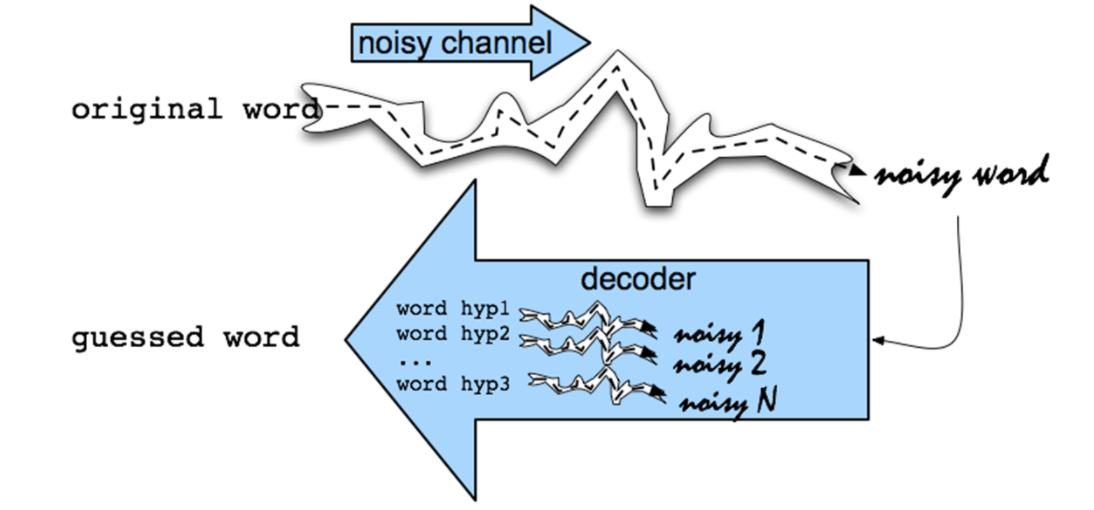
\includegraphics[width=10cm]{NoisyChannel.png}
	\caption{Noisy channel}
	\label{fig:noisychannel}
\end{figure}

\textbf{FIXME}: When for a input typo we do not have any candidate ?? 


\subsection{Common Errors}
The following type of errors were considered:
\begin{itemize}
	\item \textsc{transposed adjacent characters}
	\item \textsc{omitted digit}
	\item \textsc{additional digit}
	\item \textsc{substituted digit}: this is the probability to type a
	character $i$ when the character $j$ was intended ($P(i|j)$). This 
	probability was determined experimentally. \textbf{FIXME}: how? from where?
\end{itemize}

\section{Most Likely State Sequence}

The Viterbi algorithm calculates the most probable sequence of hidden states, the words intended.

The initial probability of being in a state $i$, $\pi_i$, in our case the probability of intend a word $i$, and the 
transition probabilities $A_{ij}$, or the transition from the word $i$ to the next word $j$, are given. Since we have 
observed the output $y_1, y_2, \dots , y_t$, that is the sentence written with typos, it is possible to computed the most 
likely state sequence $x_1, x_2, \dots , x_t$, the sentence intended, starting from the following expression:

\begin{equation}
	\begin{aligned}
		V_{1,t+1} &= P(x_1, \dots, x_t, x_{t+1}, y_1, \dots, y_t,  y_{t+1}) = \\
						&= \arg\max_{x_{1:t}} p(x_1, \dots, x_t | y_1, \dots, y_t) = \\
						& =  \alpha \cdot p(y_{t+1}|x_{t+1})\cdot\max_{x_t} \Big( p(x_{t+1}|x_t) \max p(x_1, \dots, x_{t}|y_1, 
						\dots, y_t)\Big)
	\end{aligned}
\end{equation}

%FIXME
The initial state probabilities $\pi$ are actually the word frequencies (? We don’t estimate it in a proper way), the state 
transition probabilities are given by the probability of a word given its predecessor, and the emission probabilities are the 
probabilities to type word $i$ when word $j$ was intended.

In our implementation, we construct the \textit{trellis} choosing the locally/globally best state. As we can see in the 
picture below, we display an example of the trellis drawing only the best predecessor of each state.

\begin{figure}[H]
	\centering
	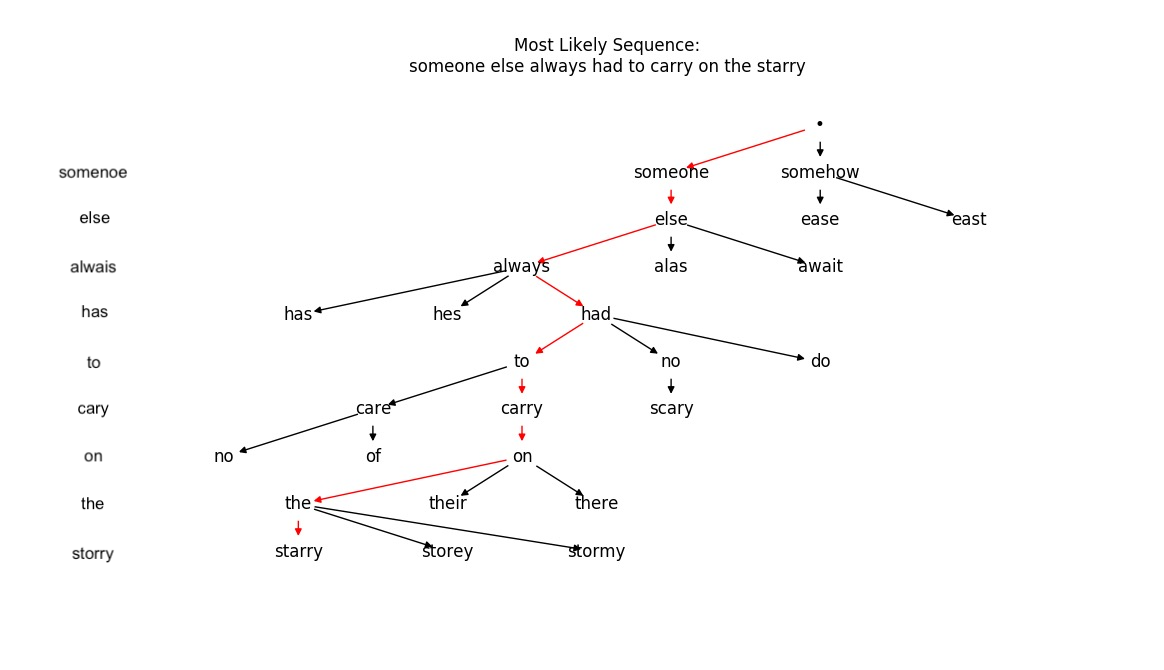
\includegraphics[width=10cm]{TrellisExample.png}
	\caption{Trellis example}
	\label{fig:trellis}
\end{figure}

In this example, we observed the sentence \textsl{my practice iu never iery absorcing} and our algorithm return the most 
likely state sequence \textsl{may practice is never very absorbing}. In this case, the algorithm partially fails, because the 
intended sentence was \textsl{my practice is never very absorbing}.
\\
\textbf{FIXME}: (pi la probabilità iniziale del prima stato non lo abbiamo, non lo facciamo perchè dal nostro dataset non 
abbiamo sempre la prima parola…)

We decide to implement the \textbf{Viterbi} based algorithm instead the Forward-Backward algorithm relying on the 
experiments carried out in the literature.
The HMM-Based Error Correction Mechanism for Five-Key Chording Keyboards article \cite{tarniceriu2015hmm} explains 
that the Forward-Backward algorithm estimates the most likely state for each observation, but the resulting state 
sequence may not be a valid succession of words in natural language (or a very unlikely word sequence) and produce 
inferior results.

\section{Myers' Algorithm}


\section{Hidden Markov Model}


\textbf{FIXME}: Hmm approach
\textbf{FIXME}: description of hmm

\textbf{FIXME}: our application ...